\section{Setting of the learning problem}

\subsection{Learning problem definition}

Can be defined as 3 components:
\begin{itemize}
	\item
	      A \iemph{generator} \(G\) of random data \(x\) from a
	      probability distribution \(P(x)\) which is fixed and unknown to us.
	\item
	      A \iemph{supervisor} \(S\) which returns an output value ${y \in Y}$
	      for every input \(x \in X\) according to a conditional
	      probability distribution \(P(y \mid x)\), also fixed and unknown
	      to us.
	\item
	      A \iemph{learning machine (algorithm)} \(L\) which is capable of
	      implementing(computing) any of a set of functions (models).
	      \(f_\theta\) where \(\theta\) is a set of parameters belonging to the
	      parameter space \(\theta\).
\end{itemize}

\begin{center}
	\tikzstyle{block} = [draw, rectangle, minimum height=3em, minimum width=3em]
	\tikzstyle{virtual} = [coordinate]
	\begin{tikzpicture}[>=stealth, auto, node distance = 1cm and 3cm]
		% Place nodes
		\node [block] (G) {$G$};
		\node [block, right=of G] (S) {$S$};
		\node [block, below=of S] (L) {$L$};
		\node [virtual, right=of S] (So) {};
		\node [virtual, right=of L.340] (Lo) {};
		\node [below right=of L, align=center] (d) {$L(y,\,\ddot{y})$ \\ (discrepancy)};

		\draw [->] (G.east) -- node [name=x] {$x$} (S);
		\draw [->, rounded corners] (x) |- (L);

		\draw [->] (S) -- node [name=y] {$y$} (So);
		\draw [->, rounded corners] (y) |- (L.20);

		\draw [->] (L.340) -- node[below] {$\ddot{y}$} (Lo);

		\draw [->, rounded corners] (d.west) -| node[below] {modify} (L.south);
	\end{tikzpicture}
\end{center}

The selection of the best possible model according to \(L\) is done
based on a learning data sample
\(D = \bigl\{(x_1,\, y_1),\, (x_2,\, y_2),\, ...,\, (x_n,\, y_n)\bigr\}\) (where \(x_i\) are
vectors)

\subsection{Why is the relation between X and Y stochastic?}

In most of the cases, randomness is ignorance of the true effects.
\begin{enumerate}
	\item
	      Ignorance of the functional dependence on a not measured variable
	      \(z\).
	\item
	      Technical invisibility.
\end{enumerate}

\subsection{Some definitions}

\begin{definition}{Loss function}{}
	A function
	\(L: Y \times Y \longrightarrow \mathds{R}+\) such that:

	\begin{align*}
		L(y,\, y') & = L(y',\, y) \tag{symmetry} \\
		L(y,\, y') & = 0  \Longleftarrow y = y'
	\end{align*}

	Examples of loss functions:

	\begin{align*}
		L(y,\, y') & := \begin{cases}1 \quad \text{if } y \neq y' \\ 0 \quad \text{otherwise} \end{cases} &  & \text{(0-1 loss) / (zero-one) / } L_{01} \\
		L(y,\, y') & := (y - y')^2                                                                        &  & \text{(squared error)}
	\end{align*}
\end{definition}

\begin{definition}{Hypothesis space}{}
	\begin{equation*}
		\mathcal{F} = \bigl\{f_\theta: \mathcal{X} \rightarrow \mathcal{Y} \mid \theta \in \varTheta \subseteq \mathds{R} \bigr\}
	\end{equation*}
\end{definition}


\begin{definition}{Classifier}{}
	Is a function \(f: X \longrightarrow Y\)
	where \(Y\) is a set of different symbols.
\end{definition}

\begin{definition}{Risk}{}
  \index{risk}\index{expected loss}\index{generalization error}\index{true error}
	The risk of a function is its \emph{expected loss}. Also known as true
	error or generalization error.

	\begin{equation*}
		\mathds{R}[f] := \mathds{E}_{(x,\, y) \sim p} \left[ L(f(x),\, y) \right]
	\end{equation*}

	\begin{note}
		A function that takes a function as an argument is called a functional.

    Risk is a functional. \index{functional}
	\end{note}
\end{definition}

\begin{definition}{Empirical error}{}\index{empirical error}

	The average error or loss function evaluated on a specific data sample
	\(D\).

	\begin{equation*}
		\hat{R}_{D^n}[f] = \frac{1}{n} \sum_{i=1}^n L(f(x_i), y_i)
	\end{equation*}

	\begin{note}
		This is also a functional.
	\end{note}
\end{definition}

\begin{definition}{Training error}{}
	The \iemph{empirical error} obtained in the data
	sample used for training.
\end{definition}

\begin{prop}{Model error proposition}{}

	For a fixed model \(f_θ\) the expected value of the
	empirical error based on a data sample is equal to the true error.

	\begin{equation*}
		\mathds{E}_{D^{ijd}p^n}[\hat{R}_{D^n}[f]] = R[f]
	\end{equation*}

	\begin{proof} TODO
	\end{proof}
\end{prop}


\subsection{Discriminative vs generative classifiers}

\begin{definition}{Discriminative classifier}{discriminative}\index{discriminative}
	A classifier that directly models the conditional probability
	\(P(y | x)\) of the output given the input.

	\paragraph{Example:} Logistic regression
\end{definition}

\begin{definition}{Generative classifier}{generative}\index{generative}
	A classifier that models the joint probability distribution
	\(P(x, y)\) of the input and the output.

	\paragraph{Example:} Naïve Bayes
\end{definition}

\subsection{Risk minimizers}

\begin{align*}
	R[f] := \mathds{E}_{(x, y) \sim p} [ L(f(x), y) ] \\
	\int_{\mathds{R}^d} \int_{\mathds{R}} L(f(x), y) p(x, y)\; dy\, dx
\end{align*}

\begin{prop}{}{}

	The function minimizing the risk on the zero-one loss is the Bayes
	classifier. Which is the one that given x, assigns the class with the
	highest posterior probability.

	\[f^* = \argmax {P(w | x)}\]

	\begin{enumerate}
		\item The risk of \(f_{01}^*\) is the Bayes risk.
		\item The upper bound of the Bayes risk is 0.5
	\end{enumerate}

\end{prop}

\subsection{Regression under the square error / loss function}

\subsubsection{Standard setting of the regression problem}

\begin{align*}
	y & = f_\text{sq.}(x,\, z)                         \\
	  & \downarrow (z \text{ is absent from the data}) \\
	y & = f_\text{sq.}(x) + \varepsilon
\end{align*}

Where:
\begin{itemize}
	\item \(\mathds{E}[\varepsilon] = 0\) (expected value of the error is 0)
	\item \(\text{Var}[\varepsilon] = \sigma^2 < \infty\) (variance of the error is finite) (a.k.a. homoscedasticity)
	\item No assumption of gaussianity
\end{itemize}

\begin{prop}{}{}
	\begin{align*}
		R[f]                       & = \sigma^2 + \int_{\mathds{R}^d} (f(x) - f^*_{sq.}(x))^2 p(x)\; dx
		                           &                                                                    & (\text{MSE}[f])              \\
		\text{where } f^*_{sq.}(x) & = \int_{\mathds{R}} y\cdot p(y(x))\; dy
		                           &                                                                    & \text{(regression function)} \\
		\text{in terms of statistics: }                                                                                                \\ \mathds{E}_{Y|x}[y | X = x] \\
		\Rightarrow R[f^*_{sq.}]
	\end{align*}

	We cannot compute this in practice since we do not know the distribution
	of the data.
\end{prop}

\begin{prop}{bias-variance decomposition}{}
  \index{bias-variance decomposition}

	The bias / variance decomposition of the mean squared error.

	\[MSE[f] = Bias(f)^2 + Var(f)
	\]

	There is a trade-off between bias and variance, known as the
	\emph{bias-variance dilemma}.
\end{prop}

\paragraph{Remainder}

Given a dataset \(D = {x^i, y^i}\) of size \(n\) \((x^i, y^i)\sim p\) We
choose a loss function \(L\) and a hypothesis space \(F\).

\[F := { x \rightarrow f_\theta(x),\quad \theta \in \Theta }
\]

\subparagraph{Observations}

The set of functions we chose matters a lot. In some sense \(F\) should
be large to minimize the chances that the chosen function is not in
\(F\).

\begin{itemize}
	\item
	      Choosing a Machine Learning Algorithm of \(F\) given a particular
	      \(D_n\) obviously depends on this \(D_n\):

	      \[D_n! \rightsquigarrow f_\theta = f_n\]
	\item The best possible solution \(f^*_{sq.}\) may not belong to \(F\).

	      In case \(f^*_{sq.} \notin F\) then we should find:
	      \(\hat{f}_{sq.} = \argmin {\lVert f - f^*_{sq.} \rVert}\)
	      We could use different norm functions.
\end{itemize}

The expression being integrated is:

\[\left( f_m(x) - f^*_{sq.}(x) \right)^2
\]

Expected value of the model for all possible datasets in \(D_n\):
\begin{align*}
	\mathds{E}_{D_n} \left[ f_n(x) \right] & =: \overline{f_n}                                               \\
	\left( \left( f_n(x) - \overline{f_n} \right) + \left( \overline{f_n} - f_{sq.}^*(x) \right) \right)^2 = \\
	\left( \overline{f_n}(x) - f_{sq.}^*(x) \right)^2 +
	\mathds{E}_{D_n} \left[ \left( f_n(x) - \overline{f_n}(x) \right)^2 \right]
	\rightarrow \text{Var}(f_n(x))
\end{align*}
How the prediction coming from a specific data sample $D_n$ varies around its mean
(Dependence of the model being learned on the specific data sample)

\(\text{Bias}^2(f_n(x))\) : how the average prediction over all possible
\(D_n\) at point \(x\) differs from the best possible prediction.

\begin{align*}
	\text{Bias}^2(f) & = \int_{\mathds{R}^d} \left( \overline{f_n}(x) - f_{sq.}^*(x) \right)^2 p(x)\; dx                           \\
	\text{Var}(f)    & = \int_{\mathds{R}^d} \mathds{E}_{D_n} \left[ \left( f_n(x) - \overline{f_n}(x) \right)^2 \right] p(x)\; dx \\
	\text{MSE}[f]    & = Bias(f)^2 + Var(f) + \sigma^2
\end{align*}

where \(\sigma^2\) is the variance of the noise.

Since \(\sigma\) cannot be reduced, it is called irreducible error. The
rest is called reducible error. \index{irreducible error}

Getting better data we reduce the irreducible error. (ignorance)

\section{Consistency}\index{consistency}

We depart from a specific data sample \(D_n\) The training error of a
model \(f\) is:
\begin{equation*}
	\hat{R}_n^{[f]} := \frac{1}{n} \sum_{i=1}^n L(f(x^i),\, y^i)
\end{equation*}

So, when we learn a specific model \(f_n\) from \(D_n\) its
\emph{training error} is \(\hat{R}_n(f_n)\) The true error of \(f_n\)
is \(R(f_n)\)

The \iemph{Empirical Risk Minimization} (ERM) prescribes to minimize the
training error. \index{ERM}

\begin{description}
	\item[Consistency]
		The ERM is said to be \emph{consistent} if:

		\begin{align*}
			\hat{R}_n(f_n) & \xrightarrow[\text{infimum}_{f \in F}]{} R(f)
			\text{ as } n \rightarrow \infty                               \\
			R(f_n)         & \xrightarrow[\text{infimum}_{f \in F}]{} R(f)
			\text{ as } n \rightarrow \infty
		\end{align*}

		These convergences are in probability.
\end{description}

Graphically:
\begin{figure}[H]
	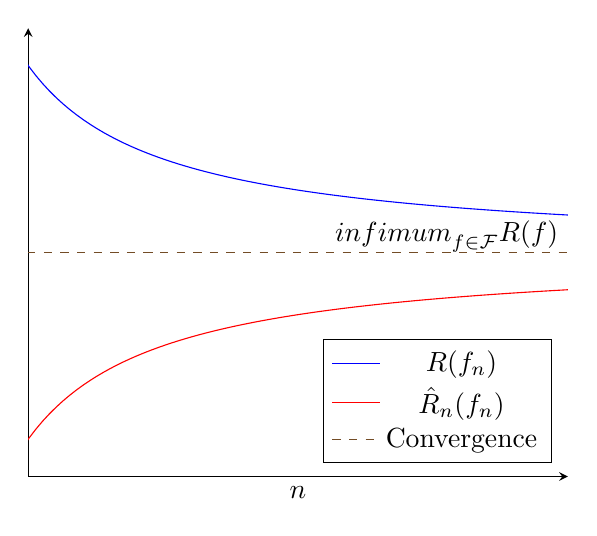
\begin{tikzpicture}
		\begin{axis}[
				domain=0.1:1.1,
				xmin=0.2, xmax=1,
				ymin=-6, ymax=6,
				samples=100,
				axis y line=center,
				axis x line=bottom,
				xlabel = {$n$},
				legend pos=south east,
				% area style,
				ticks=none,
			]
			\addlegendentry{\(R(f_n)\)};
			\addlegendentry{\(\hat{R}_n(f_n)\)};
			\addlegendentry{Convergence};
			\addplot+[mark=none] {1/x};
			\addplot+[mark=none] {-1/x};
			\addplot+[mark=none,dashed] {0};
			\node at (axis cs:1,1.1) [anchor=north east] {\(\text{infimum}_{f \in \mathcal{F}} R(f)\)};
		\end{axis}

	\end{tikzpicture}
	\caption{Convergence of the training error and the true error}
\end{figure}

\begin{theorem}{Vapnik-Chervonenkis}{}

	A necessary and sufficient condition for consistency is that the
	hypothesis space \(F\) is compact.

  % TODO: formal definition
	% \begin{equation*}
	% 	\forall \varepsilon > \dots
	% \end{equation*}
\end{theorem}
